\documentclass{article}
\usepackage{graphicx}
\usepackage{array}
\usepackage{makecell}
\usepackage{fourier}

\title{Review of Fault Tolerance Techniques in Distributed System}
\author{John Doe, Jane Doe}
\date{\today}

\begin{document}

\maketitle

\begin{abstract}
Distributed system is a collection of independent systems which can communicate with each other by transferring massages. There are some major issues in distributed systems but we focus in this paper on fault tolerance. It is the system’s ability to work in the condition when there occur any type of some fault in the system, like failure in communication, hardware or resources. It is a very important issue in distributed system, in this paper we present a survey of different types of fault tolerance techniques and their comparison.
\end{abstract}

\section{Introduction}
A Distributed system is the collection of computers which are independent and appears to its user as a single coherent system. Distributed system is linked by some local networks and they are interlinked with each other’s physically. It uses a computer network in which each computer works on some portion of overall task, in this manner a large task can be performed very efficiently and quickly than a single computer. Distributed System is much better than centralized system as it does not have any centralized controller so there is no chance of the failure in the distributed system because in distributed system computers are connected with number of servers so if one server is down it can get data from another server. It can easily extendable by adding more computers to the network. It allows many users to share data at the same time and makes man to man communication very easier. Some Examples of distributed computing systems are online Air, Railway reservation systems, air traffic control systems, Cellular network, industrial control system, banking system, wireless sensor network, multiplayer online games etc[1].

\section{Issues in Distributed Computing System}
Distributed system may have some issues and due to which its rate can be lower down. These issues can be:

\subsection{Flexibility}
The distributed system should be flexible so that the users can easily modify and enhance it.

\subsection{Scalability}
To design a system in such manner so that it can easily coping up and as a result growth of the system will increase. Central algorithms and central entities should be avoided by the system and most of the operations should be performed at the client work station by the system.

\subsection{Fault Tolerance}
The faults must be resisted by the system. If any fault may occur in future, the system performance doesn’t degrade. The factors that generate faults in the system can be mobility, load imbalance, overloading and many more[1].

\subsection{Security}
The various resources of the system must be secured from unauthorized access and destruction so that the users can trust them. Due to the usage of insecure networks for data communications and the lack of its control from the single point, the provision of security in the distributed system is more difficult than in the centralized system[2].

As Now a days the size of distributed systems are increasing very rapidly day by day as the number of users are increasing, so the chance of problems and errors in the distributed systems is also increasing. Millions of devices are working together and are prone to failures. Some examples of failures are memory, power, disks, processors and link failure. Diagnosing the faults in large distributed system is very difficult. It may halt or stop the normal working of distributed system and may turn the whole system execution in wrong path. In different reservation systems, internet banking, or in air traffic control system a single fault can give a very large amount of loss

\section{VARIOUS FAULT TOLERANCE \\ TECHNIQUES}
We will discuss different fault tolerance techniques in this paper.

\subsection{Replication Based Fault Tolerance Techniques}
Replication based fault tolerance technique is one of the famous fault tolerance techniques. The word replica originates from the repetition and it means multiple copies. Replication is the process of maintaining different copies of same object or data item. In replication technique, client request is forwarded to one of replica among a set of replicas[2]. This replication technique is used for that request of client which will not alter the service state. Replication adds redundancy in the system. In this way if some of nodes fails to do work it will not result in the failure of the whole system and thus the fault tolerance is achieved as shown in fig \ref{1}

\begin{figure}
    \centering
    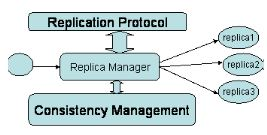
\includegraphics[width=0.47\textwidth]{../figz/replication}
    \caption{Replication Based Technique}
    \label{fig:1}
\end{figure}

Although Replication is a very good technique for fault tolerance but in this technique there are some issues that are Consistencies among all of the replica, replica on demand, replica management, degree of replica etc. We have discuss here consistency and degree of replica.

\subsubsection{Consistency}
Consistency among replicas is the big issue in replication fault tolerance technique. Multiple copies of same data/entity causes the problem of consistency, the reason is update of any copy by any one of the users. A replication protocol must ensure the consistency between all of the replicas of the same object or entity. Consistency is ensured in this replication technique by some of the criterion. Many criteria for consistency have been defined such are sequential consistency and linearizability. In both the cases, an operation is performed on the most recent state of the object. Sequential consistency informally states that a multiprocessor program executes correctly if its result could have been produced by executing that program on single processor system. In order to have consistency an efficient strategy is required. Passive strategy and active strategy are main strategies. In a passive replication, only one primary execute requests and multicasts state changes to all replicas. This scheme avoids redundant computation of requests. It copes with non-deterministic service behavior. In active replica, client request is multicasts to all replicas. This means all replicas execute the request individually. In this way active replica takes less network resources than sending update. Active replica response to a fault is faster than passive. However, replica consistency usually requires deterministic replica behavior.

\subsubsection{Degree of Replica}
Number of replica is known as a degree of replication. In order to replicate an object a replication protocol is used. Primary-backup replication, voting, and primary-per partition protocol are some of the replication protocol. A replication protocol must be practical and simple. Niobe is such protocol purposed by researcher. Number of replicas must be sufficient. Large numbers of replicas will increase the cost of maintaining the consistency. Less number of replicas will affect the performance, scalability and multiple fault tolerance capability. Therefore, reasonable number replicas must be estimate as per system configuration and load. Researcher proposed adaptive replicas creation algorithm. There is further research scope to develop improved algorithm to maintain a rational replica number. Replica on demand is a feature that can be implemented to make more adaptive, flexible and dynamic.

\subsection{Check pointing and Roll Back}
Checkpoint with rollback-recovery is a well-known technique. Checkpoint is an operation which stores the current state of computation in stable storage. Checkpoints are established during the normal execution of a program periodically. This information is saved on a stable storage so that it can be used in case of node failures. The information includes the process state, its environment, the value of registers, etc. When an error is detected, the process is roll backed to the last saved state. Fig \ref{fig:2} shown below gives an idea about this technique

\begin{figure}
	\centering
	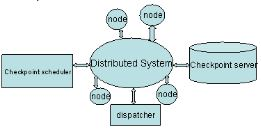
\includegraphics[width=0.47\textwidth]{../figz/check}
	\caption{Check Pointing Technique}
    \label{fig:2}
\end{figure}

Basically this technique is used to restore the process to certain point after failure occurs. Fault Tolerance can be achieved through various types of redundancy. Check-point start is the common method. In this method an application starts from the earlier checkpoint after a fault. Application may not be able to meet strict timing targets[2].

\subsection{Fusion Based Technique}
Although replication method is widely used as a fault tolerance technique but number of backups is a main drawback. Number of backups increases drastically as coverage against number of faults increases. As the number of backup increases management of these backups is very costly. Fusion based techniques overcome this problem. It is emerging as a popular technique to handle multiple faults. Basically it is an alternate idea for fault tolerance that requires fewer backup machines than replication based approaches. In fusion based fault tolerance a technique, back up machines is used which is cross product of original computing machines. These backup machines are called as fusions corresponding to the given set of machines. Overhead in fusion based techniques is very high during recovery from faults. Hence this technique is acceptable if probability of fault is low.
Fig \ref{fig:3} below gives a basic idea about fusion

\begin{figure}[ht]
\centering
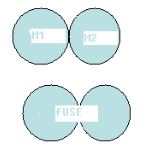
\includegraphics{../figz/fault}
\caption{Fusion Based Technique}
\label{fig:3}
\end{figure}

\section{Comparison}
From the comparison it is clear that all methods having capability to handle multiple faults. In all methods performance can be improved by addressing the critical factors involved. In all techniques there is strong need for reliable, accurate and pure adaptive multiple failure detector mechanism. 

\section{CONCLUSION}
\begin{table}[h]
    \centering
    \caption{A brief summary of the previous content}
    \label{t1}
    \begin{tabular}{ | c | c | c | c | }    
        \hline
        \thead{Major\\Factors} & \thead{Replication\\Based} & \thead{Check\\point} &\thead{Fusion\\Based} \\
        \hline
        \small{Working}& \makecell{\small{Request is}\\\small{redirected}\\\small{to replica}}& \makecell{\small{State saved} \\\small{on Stable} \\\small{storage Used}\\\small{for recovery}}&\makecell{\small{Back up}\\\small{machine}} \\
        \hline        \small{Consistency}&\makecell{\small{Linearizi}\\\small{bility,}\\\small{Sequential}}& \makecell{\small{avoiding} \\\small{updated} \\\small{messages}}&\makecell{\small{Among}\\\small{Back up}\\\small{machine}} \\        
        \hline    		\makecell{\small{Multiple}\\\small{Faults}\\\small{Handling}}&\makecell{\small{Depends}\\\small{upon No}\\\small{of Replica}}& \makecell{\small{Depends} \\\small{upon}\\\small{Checkpoints}\\\small{Scheduling}}&\makecell{\small{Depends}\\\small{Upon}\\\small{No of}\\\small{machines}} \\
    	\hline
    \end{tabular}
\end{table}

Fault tolerance consists of two major components; failure detection and recovery. In this we have identified important issues such as fast, adaptive, accuracy, completeness, confidence and able to detect multiple faults. A reliable detector must not suspect a working process or processor and at the same time, it must detect all faults as early as possible. Multiple faults with performance is future trends of fault tolerance techniques Performance of a multiple fault tolerance algorithm depends on how much algorithm is capable to prevent the further loss due to faults.

\section{Refrences}
%% 이런 형태의 참고문헌은 글쎄..?
\begin{enumerate}
  \item Alfred~V. Aho and Jeffrey~D. Ullman. 1972. The Theory of Parsing, Translation and Compiling, volume~1. Prentice-Hall, Englewood Cliffs, NJ.
  \item American Psychological Association, 1983, Publications Manual, American Psychological Association, Washington, DC.
\end{enumerate}

\end{document}